\section{SMAD: SMart Aggregation of Anti-patterns Detectors}
\label{section: smad}
\subsection{Problem Definition}
Let us consider $D$ anti-patterns detection tools $d_{1},d_{2}, ..., d_{D}$ performing a boolean prediction over the entities (i.e., classes or methods) of a software system based on some internal detection rule. We refer to as $d_{i}(e) \in \{True, False\}$ the boolean prediction of the $i^{th}$ detection tool on an entity $e$.

We want to combine these approaches to maximize the Matthew's Correlation Coefficient (MCC) (cf. Equation~\ref{mcc}) of the so-produced ``merged'' prediction over the entities of the studied system. Thus, we want to find a function of the $D$ approaches that outputs an improved prediction on any software system $S$. Which can be expressed as:

\[f(d_{1},d_{2}, ..., d_{D}, e) \in \{True, False\}\] 
and 
\[MCC(f(d_{1},d_{2}, ..., d_{D}, S)) \geq \maxx_{i} MCC(d_{i}(S)), \quad \forall S\]

\subsection{Overview}
\label{subsection: overview}
The proposed method \NAME{} allows to combine various detection approaches on the basis of their internal detection rule instead of their output. Indeed, the internal detection process of any rule based approach relies on some structural or historical metrics (i.e., core-metrics) that can be computed for any entity to be classified. Thus, the key idea behind \NAME{} is to compute the core-metrics of various approaches for each input entity and use these metrics to feed a machine-learning based classifier. First, for each anti-pattern considered in this study, we selected three state-of-the-art detection tools to be aggregated. These tools respectively rely on:

\begin{itemize}
\item \textit{Rule Cards:} Affected entities are identified using a combination of source-code metrics designed to reflect the formal definition of the anti-patterns. For this category, we selected DECOR \cite{Moha10-TSE-DECOR} for God Class and InCode \cite{marinescu2010incode} for Feature Envy detection.  

\item \textit{Historical Information:} Affected entities are identified via an analysis of change history information derived from versioning systems. For this category, we used HIST \cite{PalombaBPOLP13,Palomba15} for both God Class and Feature Envy detection.

\item \textit{Refactoring Opportunities:} Anti-patterns are detected by identifying the opportunities to apply their corresponding refactoring operations. For this category, we used the refactoring operations Extract Class \cite{fokaefs2012identification} and Move Method \cite{tsantalis2009identification} provided by JDeodorant, respectively for God Class and Feature Envy detection.
\end{itemize}

Selecting tools that are based on different strategies allows us to expect a high complementarity of the aggregated approaches and thus, maximize the expected performances of our method. Then, we selected the core metrics, i.e., metrics that reflect best the internal decision process of each tool, as input features for our model. The classifier used by \NAME{} to predict whether an entity is an anti-pattern or not is a Multi-layer Perceptron (MLP), i.e., a fully-connected feed-forward neural-network. This model is composed of \textit{tanh} dense hidden layers connected to a \textit{sigmoid} output layer. Fig.~\ref{fig: smad} overviews our approach. 


\begin{figure}[htb]
\centering
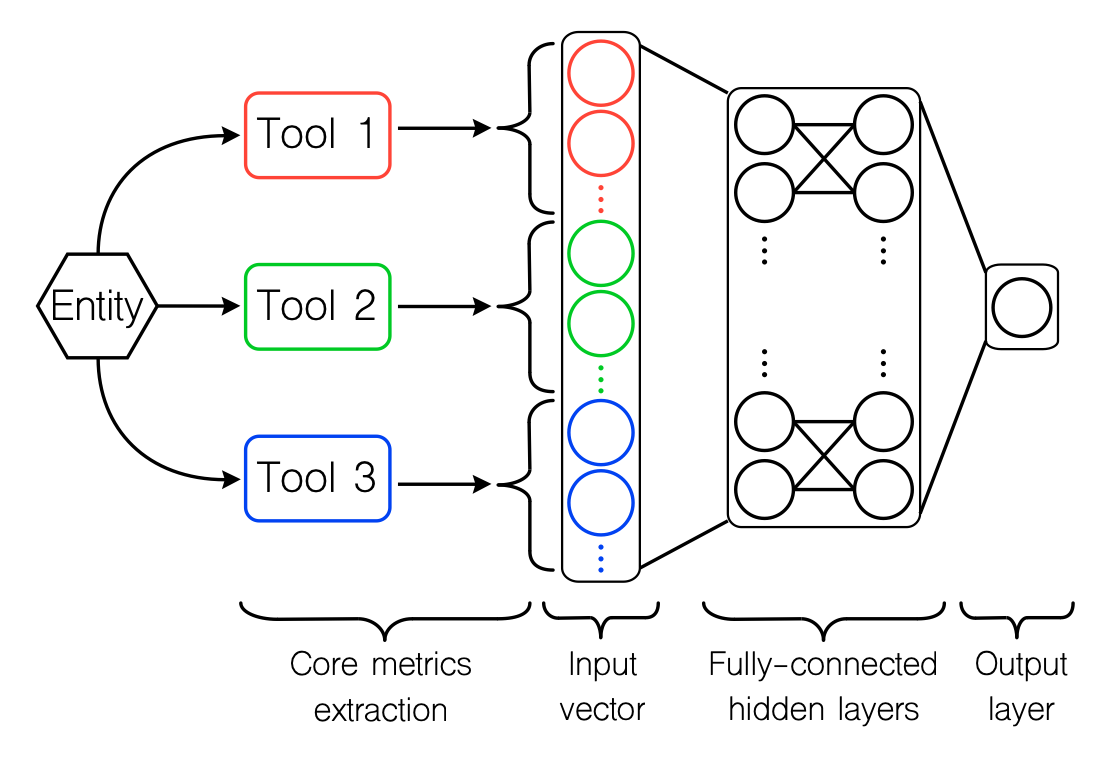
\includegraphics[width=9.2cm]{images/SMAD}
\caption{Overview of SMAD Detection Process}
\label{fig: smad}
\end{figure}

\subsection{Input}
\label{subsection: input}
\subsubsection{Metrics for God Class Detection}

For God Class detection, we extract \textbf{six} core metrics from the three detection tools considered in this study. These metrics are computed for each class of a system.


\paragraph{DECOR:}
The internal detection rule relies on the definition of four code and design smells and can be expressed as: ``(is associated to many \textit{DataClass}) AND is a (\textit{ControllerClass} OR \textit{LargeClass} OR \textit{LowCohesionClass})''. These smells are defined using structural and lexical metrics along with some thresholds: (1) \textit{DataClass} relies on the number of accessors, (2) \textit{ControllerClass} relies on lexical properties, (3) \textit{LargeClass} relies on the  sum of the NMD and NAD metrics (Number of Methods Declared + Number of Attributes Declared), and (4) \textit{LowCohesionClass} relies on the LCOM metric (Lack of Cohesion in Methods) \cite{briand1998unified}. Thus, we extracted four core metrics from DECOR internal detection rule for God Class:
\begin{itemize}
\item  Number of associated \textit{DataClass}
\item $\llbracket$\textit{ControllerClass}$\rrbracket$
\item nmd\_nad
\item lcom 
\end{itemize}

\noindent with $\llbracket \rrbracket$ a boolean variant of the kronecker delta defined in Equation~\ref{kronecker}, nmd\_nad and lcom are the uppercase metrics divided by their respective threshold. The value of these thresholds depends on the systems characteristics and can be computed through the Ptidej API~\footnote{https://github.com/ptidejteam/v5.2}.

\paragraph{HIST:}
God Classes are identified as: ``classes modified (in any way) in more than $\alpha$\% of commits involving at least another class''. Thus, we extracted one core metric from HIST internal detection rule for God Class:
\begin{itemize}
\item  Ratio between the number of commits in which the considered class has been modified along with other classes and the number of commits involving other classes of the system.
\end{itemize}

\paragraph{JDeodorant:}
God Classes are classes from which a \textit{concept} (i.e., a subclass) can be extracted. Formally, a concept is defined as: ``a distinct entity or abstraction for which a single class provides a description and/or a set of attributes and methods that contribute together to the same task''. We define our core metric for JDeodorant as:
\begin{itemize}
\item  Number of \textit{concepts} that can be extracted from the considered class.
\end{itemize}

\subsubsection{Metrics for Feature Envy Detection}
\label{Paragragh: metrics feature envy}

A Feature Envy is characterized by two source code components: a method (i.e., the envious method) and a class (i.e., the envied class). Hence, in a given system, the number of potential entities that must be investigated is equal to $n_{m}\times(n_{c}-1)$ with $n_{c}$ and $n_{m}$ respectively the numbers of classes and methods in the system. To reduce this number, we filter the studied system at both class and method level, similarly to Tsantalis and Chatzigeorgiou~\cite{tsantalis2009identification}. First, we consider as potential envious methods only non-static and non-accessor methods. Then, for each of the remaining methods, we consider as potential envied classes only classes that are accessed in some way in the body of the method. We extract \textbf{seven} core metrics from the three considered detection tools.

\paragraph{InCode:}
Methods are identified as being envious without information about the envied class. In this context, a method is declared affected if: (1) ``it uses directly more than a few attributes of other classes'' (ATFD $>$ FEW), (2) ``it uses far more attributes from other classes than its own'' (LAA $<$ ONE THIRD), and (3) ``the used “foreign” attributes belong to very few other classes'' (FDP $\leq$ FEW). We redefined the first two metrics to express information about the envied class, which led us to three core metrics:
\begin{itemize}
\item ATFD (Access To Foreign Data), i.e., number of attributes of the envied class accessed by the method.
\item LAA (Locality of Attribute Accesses), i.e., ratio between the number of accesses to attributes that belongs to the envied class vs.\ the enclosing class.
\item FDP (Foreign Data Providers), i.e., number of distinct foreign classes whose attributes are accessed by the method. 
\end{itemize}

\paragraph{HIST:}
Feature Envy methods are identified as: ``methods involved in commits with methods of another class of the system $\beta$\% more than in commits with methods of their class''. Thus, we extract one core metric from HIST internal detection rule for Feature Envy:
\begin{itemize}
\item Ratio between the number of commits involving the considered method and methods of the envied class vs. methods of the enclosing class. 
\end{itemize}

\paragraph{JDeodorant:}
For each method $m$ in the system, a set of candidate target classes $T$ is created and sorted based on: (1) the number of entities (methods or attributes) that $m$ accesses from each class of $T$ and (2) the Jaccard distance (cf. Equation~\ref{jaccard entity to class}) between $m$ and each target class. Then, JDeodorant suggests to move $m$ to the first target class that satisfies a set of preconditions related to compilation, behavior, and quality. We extracted three core-metrics, which can be expressed as:
\begin{itemize}
\item Ratio between the number of accesses to entities that belong to the envied class vs.\ enclosing class.
\item Ratio between the Jaccard distance from the method to the envied class vs.\ enclosing class.
\item Boolean value indicating whether the Move Method Refactoring operation has been proposed by JDeodorant or not.
\end{itemize}

\subsection{Replication Package}
To facilitate further evaluation and reuse of our work, all the data used in this study is publicly available\footnote{https://github.com/antoineBarbez/SMAD/}. Our replication package includes: (1) the oracle; (2) the source code of our model; (3) the scripts used to generate our data; and, (4) the implementation of our experiments. Furthermore, we created a component called \textit{repositoryMiner} to extract automatically all the necessary data to test or train our model on new systems.